\chapter{Introduction}
\label{Basics of File System}
%\section{Introduction}
\section{Minix}
Minix was initially developed for educational purposes by Prof. Andrew
Tanenbaum.
Minix 3 has a highly reliable, secure and flexible microkernel OS. A minimal kernel provides 
\begin{itemize}
\item interrupt handlers
\item a mechanism for starting and stopping processes
\item a scheduler
\item interprocess communication
\item deadlock detection
\end{itemize}

The \emph{file system}, \emph{device drivers}, \emph{the network server} and \emph{high level memory management} run as appropriate user processes that are encapsulated in their private address space.

\emph{Reincarnation server} is an important one in minix. It helps in recovering from failures. Servers and drivers are started and guided by it. If a guarded process unexpectedly exits or crashes, this is immediately detected - the reincarnation
server is notified by the process server and the process is automatically restarted. It also periodically polls all servers and drivers for their status.
If one doesn't respond correctly within a specified time interval, the
reincarnation server kills and restarts the misbehaving server or driver.
%INSERT IMAGE 
\begin{figure}[!htb]
    \centering
    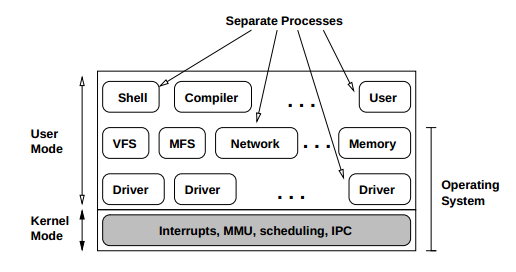
\includegraphics[scale=0.5]{img/fourlevel.png}
    \caption{Minix Layred Structure}
\end{figure}

\section {Immediate File System}

In minix, the \emph{metadata} of a file is stored in form of inodes.
Inodes contain information such as last access time, modification time, file
size, permissions etc. along with the pointers to the disk block where the data of a file is stores.
These pointers either directly refer to a disk block,
or they refer to a block that stores a list of additional pointers to data blocks
(such pointers are called indirect). 
The problem with a regular file is that even when it is very short,
a complete disk block needs to be allocated. This wastes disk space.

In immediate files, the data is stored directly in the inode instead of the
disk. An inode in Minix is 64 bytes long, and 40 bytes are used to hold pointers to data blocks.
When no data blocks are used, these 40 bytes can be used to store the file
content directly.
% IMAGE OF INODE
Thus, for files up to 40 bytes, immediate files work and hence getting rid of
fragmentation.
 Another important thing about immediate files is that the number
of disk accesses is reduced for short files and hence reducing the access time.
 

\section{File System in Minix}
In minix, File System is basically a network file server that happens to be running on the same machine as the caller.
The communication between various absract layer is via messages.
Messages from user include - \emph{access, chdir, chmod, chown, chroot, close, creat} etc system calls.
The main program in the file system waits for new messages to arrive and handles
the work according to the parameters passed in the message. There are  six sections within the Minix File System:
\begin{itemize}
\item \emph{Blank Block} – first block is reserved for boot code information
\item \emph{Super Block} – second block stores the Super Block, or information about the Minix File System
\item \emph{Inode Map} – section made up of bits, where one bit represents one inode. Tracks used and unused inodes.
\item \emph{Zone Map} – section made up of bits to track used and unused zones. %DEFINE ZONES
\item \emph{Inode Table} – manages file and device information
\item \emph{Data Zone} – majority of volume which contains files and directories.
\end{itemize}

 \newpage

 \section{File System in Minix 3.2}
 The file system in minix is more modular than the earlier versions because of
 inclusion on Virtual File System. It makes the access to the file systems 
easier by providing a uniform interface. When any file operation is to be done,
first a call is made from the user program to the virtual file system, which
consecutively passes in to the appropriate file system.

 

\subsection{Virtual File Systems}

All the system calls are directed to the Virtual File System, which directs them
to the appropriate File Systems using messages and setting the necessary flags.
The response from the File Systems also arrives at the VFS which sends it to the
user level programs using appropriate message formats and flag sets.
 It makes adding new file systems very easy since the interface is taken care of
 by the vfs. Roles of VFS are as follows:
\begin{itemize}
\item \emph{Handles POSIX} system calls.
\item \emph{Maintains state} - cooperates with the process manager to handle fork, exec
and exit system calls.
\item Keeps \emph{track} of endpoints that are drivers for character or block special
files.
\end{itemize}
 VFS is \emph{synchronous}. It sends a request to FS process and
waits until the response arrives. It contains data structures corresponding to almost all the data structures in File Systems.

\begin{figure}[!htb]
    \centering
    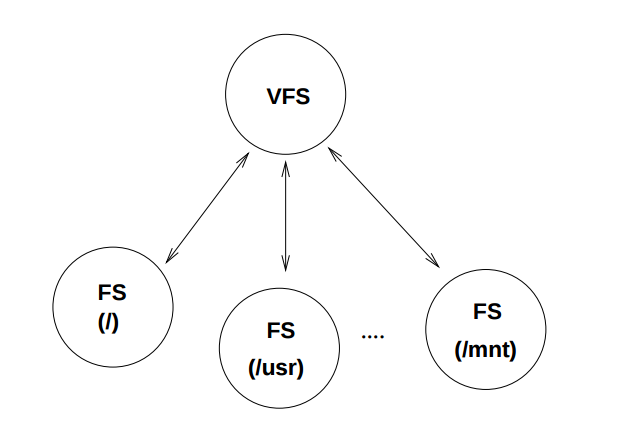
\includegraphics[scale=0.5]{img/vfslayer.png}
    \caption{VFS Layer}
\end{figure}
\begin{itemize}
\item Virtual Nodes : Vnode Object- abstract correspondence of a file. It contains
inode number of file , FS Process kernel endpoint number
\item Virtual Mounts : Vmnt Object- Store information about the mounted partitions.
\item Contains the kernel endpoint number of the File System that manages the given partition, device number, mount flags etc.
\end{itemize}

VFS spawns \emph{worker-threads} at startup. Main thread fetches requests and replies and hands them off to the idle or reply pending workers. \emph{open.c} is an important file in VFS. It contains procedures for creating,
opening, closing and seeking on files-\emph{ CREAT, OPEN, MKNOD, MKDIR, CLOSE, LSEEK} are the entry points to this call. \newline
\emph{request.c} is the file where the functions which pass on the request to file systems in proper response messages is sent.



\subsection {System Calls in MFS}
System call is how a user program requests a service from an operating system's
kernel.  Generally, systems have a library which define these system calls.
In minix, there are two components to a system call - 
\begin{itemize}
\item \emph{User Library} - Packages the parameters for system calls and calls the handler on
appropriate server.
\item \emph{System call} handler -executed in serve processes,  called in response to a user
requesting a system call.
\end{itemize}

In each server directory, there are two important files - table.c and proto.h.
\begin{itemize}
\item \emph{table.c} - contains the information regarding which file is to be called in reponse to which system call number.
\item \emph{proto.h} - declares the prototype of system call handler.
\end{itemize}
misc.c, stadir,c, write.c and read.c contain definitions for system call handler functions.

\subsection {Example: Read System Calls in MFS}
\begin{equation}
    n = read (fd, buffer, nbytes)
\end{equation}

Library procedure read is called with three parameters - file descriptor*, buffer, and number of bytes to be read. It builds a message containing these parameters along with the code for read as message type, sends the message to VFS and blocks awaiting the reply.
The VFS implementation of the system call is already explained in VFS section.

In the corresponding file system,  a procedure extracts the file descriptor from the message and uses it to locate the filp (onpen file table)) entry and then the inode. The requests are broken up into pieces such that each piece fits within a block. For each piece, chunk is made to see if the relevant block is in cache. Id not then LRU algorithm is applied.
Once the block is in cache, the file system sends message to the system task asking it to copy the data to appropriate place in the user's buffer. FS sends the reply message to the user, specifying how many bytes have been copied.

\subsection{Message passing}
There are 39 types of messages requesting work in the File System. Message
passing is basically dealt by the kernel, so, for file system purposes, we just
need to understand how to use messages. 
Different types of flags and feilds are passed via messages across different
layers of the operating sytem.
%add stuff - code format and specific files

% \newpage
% \section{Example to understand the flow of calls in VFS}
% \begin{figure}[!htb]
%     \centering
%     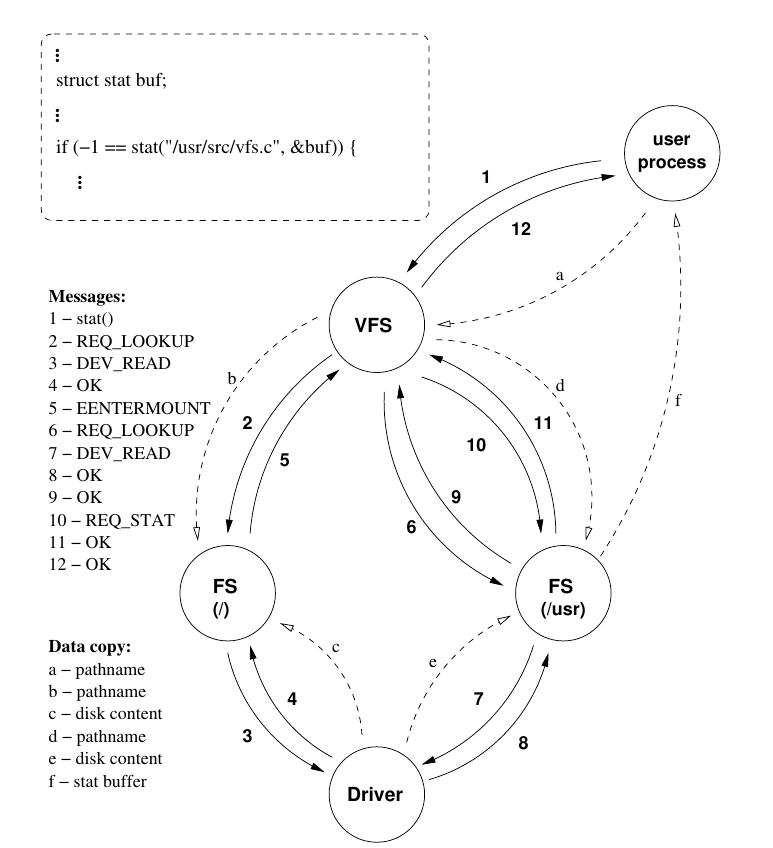
\includegraphics[scale=0.7]{img/vfsflow.png}
%     \caption{VFS Flow}
% \end{figure}




